
  
  

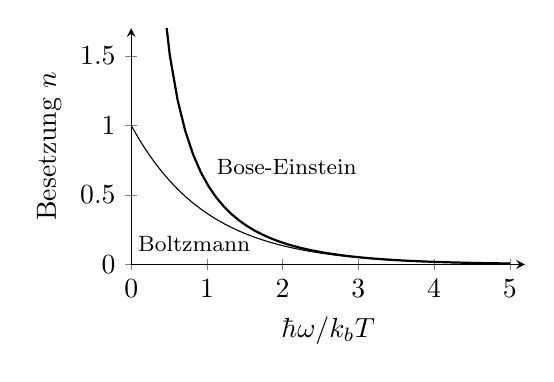
\begin{tikzpicture}

%\omega^2 =  \frac{c}{\mu}
%\pm c \sqrt{ \frac{1}{\mu^2} - \frac{4}{M_1 M_2}  \sin^2 \left( %\frac{1}{2}  \mathbf{k} \cdot \mathbf{a} \right) } 


%\useasboundingbox (0,0) rectangle (5,5);
%\draw (0,0) rectangle (5,5);



\begin{axis}[%clip=false ,
    height=3cm,
    width=5cm,
    xtick pos = bottom,
    scale only axis,
            separate axis lines,
  axis x line=bottom,
  axis x line shift=0pt,
  %xlabel shift=10pt,
  axis y line=left,
  axis y line shift=0pt,
%  ylabel shift=10pt    
 xlabel = {$\hbar \omega / k_b T$}, 
ylabel = {Besetzung $\braket{n} $},
  axis y line=left, clip=true,
  xmin = 0, xmax = 5.2,
  ymin = 0, ymax = 1.7,
%  ytick = \empty,
%  xtick = \empty,
%,ytick pos = left, ytick = {0}, 
% xmin=1320, xmax = 1520, xtick = {1415}, xticklabel = {1415}
 ]

           
% \addplot[thick]  table [x index=0, y index=1] {\currfiledir dos_si_all.dat};
 \addplot[thick, domain=0:5,samples=50]  {1 / (exp(x) -1)};
\addplot[thin, domain=0:5,samples=50]  {1 / (exp(x) )};

 \node[left] at (1.7,0.15) {\footnotesize Boltzmann};
\node[right] at (1,0.7) {\footnotesize Bose-Einstein};

 \end{axis}

\end{tikzpicture}


